This chapter is organised as a methodological pipeline that mirrors the proposed
system. An agent must learn a venue's normal trading rhythm; it must show that
the rhythm was scored on a defensible measure; it must notice when the present
departs from that rhythm; it must decide whether the departure justifies
interrupting a manager; and it must be judged on whether that decision was a good
one. Each section consumes the output of the one before it. Two are deliberately
parallel: Section~\ref{sec:rw-ruler} asks how a forecaster should be judged, and
Section~\ref{sec:rw-evaluation} asks the same of the agent built on top of it.

Four arguments run through the whole, and this review takes a position on each
rather than surveying opinion: that operational rhythm can be borrowed across
venues, though the theory of that benefit concerns large collections and its
extension to a three-venue estate is this chapter's conjecture; that a deviation
is best defined as the breach of a calibrated band, whose guarantee degrades
gracefully under a regime change rather than holding through it; that a learned
rhythm serves as the agent's model of normality, in the bounded sense
Section~\ref{sec:rw-surfacing} delimits; and that the worth of a proactive alert
turns on the asymmetric human cost of a false alarm, which is an empirical claim
with empirical support.

Two features of the evidence base are recorded here. The frontier of proactive
agency is young: eleven works cited below had not completed peer review at the
time of writing, all arXiv preprints dated between 2024 and 2026, and each is
marked at its citation. Second, this review was written after the experimental
work it introduces, so where the literature anticipates an outcome in this estate
that anticipation is an argument the reader can check against the source, not a
record of what was believed beforehand. Two places where the literature points
the other way from what this project observed are marked in
Sections~\ref{sec:rw-ruler} and~\ref{sec:rw-deviation}.

\section{Decision support and the arrival of delegated autonomy}
\label{sec:rw-framing}

The system this dissertation builds is a manager-facing agent, and a related-work
chapter must first settle what kind of artefact that makes it.
\citet{gorry_framework_1971} drew the distinction that still organises the field:
a decision is \emph{structured} when Simon's intelligence, design and choice
phases can be formalised into rules, and \emph{unstructured} when it resists
formalisation and demands human judgement, with decision-support systems
positioned to assist managers on the unstructured cases rather than replace them.
For five decades the manager remained the decision-maker and the software
remained the support. \citet{kumar_agentic_2026} argue that agentic AI breaks
this arrangement, and that what separates an agent from earlier enterprise
software is delegated autonomy: the capacity to initiate actions, make decisions
and coordinate activity toward a goal with little human prompting, so that agency
is distributed across people and machines instead of held by the user alone. Read
against Gorry, this is a different category of actor, one that participates in
the decision rather than merely informing it.

The category is already populated, and faster than it is understood. An index of
thirty widely used agentic products
\citep[a 2026 preprint]{staufer_2025_2026} documents systems acting with limited
oversight while finding that developers disclose almost nothing about safety and
evaluation, leaving no public information for 135 of 240 safety fields. The gap
is not peculiar to agents: surveying published reports of machine-learning
deployments, \citet{paleyes_challenges_2022} map the difficulties practitioners
report onto the stages of a deployment workflow and find issues at every stage.
Their catalogue is assembled from case studies of systems in use rather than
benchmark results, which is why the setting in which an agent is evaluated is
itself a variable.

This dissertation takes the position, which the chapter develops rather than
assumes, that an agent acting unasked must hold an internal model of what is
\emph{normal} for the venue it manages, because an unprompted action is warranted
only by a departure from expectation. Evidence arrives in
Section~\ref{sec:rw-surfacing}, where the dominant documented failure of
proactive systems is over-offering \citep{lu_proactive_2024}, and in
Section~\ref{sec:rw-evaluation}, where the cost of that failure falls on the
operator's willingness to keep reading
\citep{dixon_independence_2007,ancker_effects_2017}.

\section{Learning a venue's rhythm when the history is short}
\label{sec:rw-rhythm}

By a venue's \emph{rhythm} we mean its recurring pattern of trade, the
day-of-week and seasonal regularities against which a given day can be called
typical or surprising. The defining difficulty is scarcity: a single hospitality
venue offers months, not years, of clean history, and one that has just opened
offers none, which rules out the assumption of much forecasting work that each
series carries enough history to be fitted in isolation.

Within that constraint the demand-forecasting literature delivers a result that
is easy to overlook. Simple methods are hard to beat. \citet{chae_value_2024},
studying a large restaurant chain, report that deep models given only internal
operational and calendar features outperformed both their own richer variants and
most machine-learning models through the turbulent trading period, the external
macroeconomic channel paying only once conditions stabilised; their own
conclusion is that external data does help, markedly so for the machine-learning
models, and what this work inherits is the narrower recommendation they draw,
that a business without the resources to acquire external data can still forecast
competitively from operational features alone.
\citet{hossain_comparative_2025} reinforce the point from the opposite direction,
finding that classical exponential smoothing and
\citet{croston_forecasting_1972}'s method outperform a gradient-boosted baseline
on restaurant data, the boosted model failing to capture seasonality without
hand-built features. \citet{schmidt_machine_2022} report a related pattern across
twenty-three models on a single restaurant's sales, though separations at the
one-week horizon are a fraction of a percentage point on one venue with no
dispersion reported, so the study illustrates a possible horizon dependence
without evidencing one. Together these set the baseline expectation this work
inherits: on small, seasonal hospitality series, classical statistical and linear
models set a competitive bar that a more elaborate method must clear on evidence,
not on architecture.

\subsection{When does borrowing across series pay?}

The transfer route promises to relieve scarcity by importing structure learned
elsewhere, and the question is not whether that is possible but when it is worth
doing. \citet{montero-manso_principles_2021} give the clearest available answer.
Globality is not a similarity assumption: global methods are, in their words, not
more restrictive than local methods, since both can produce the same forecasts
without any assumptions about similarity of the series. What differs is where the
estimation budget is spent, since the complexity of local methods grows with the
size of the set while it remains constant for global methods, so that, and the
qualifier is the authors' own, \emph{in large datasets} a global algorithm can
afford to be quite complex and still benefit from better generalisation.

Two limits bear on the use made of that here. It is a claim about
\emph{estimation}, whereas the mechanism this work employs conditions a frozen
pretrained model on sibling series at inference time, fitting nothing on the
estate; and the formalism supplies no threshold, since nothing in it says three
series is small and forty is large. The expectation carried into these
experiments, that pooling across a three-venue estate will yield little, is
therefore an extension by analogy and this chapter's conjecture, not
\citeauthor{montero-manso_principles_2021}'s result. It is stated so that it can
fail, and the demonstrations relied on below cannot refute it, being evaluated on
established multi-series benchmarks \citep{das_-context_2025}, on a collection of
web pages \citep{zhou_context-driven_2025}, and on a mixed corpus assembled from
several public datasets \citep{liu_generative_2024}.

Time-series foundation models pretrain on large heterogeneous corpora and
forecast unseen series zero-shot, dividing by representation. TimesFM
\citep{das_decoder-only_2024} is a patched decoder predicting the next patch
autoregressively at 200M parameters; Chronos \citep{ansari_chronos_2024}
quantises real values into a fixed token vocabulary so a language-model
architecture can be trained on them, reporting zero-shot accuracy on 27 held-out
datasets comparable or superior to models trained on those series directly, and a
wider family of masked-encoder, quantile and probabilistic entrants
\citep{woo_unified_2024,liu_moirai_2026,goswami_moment_2024,rasul_lag-llama_2024,garza_timegpt-1_2024}
fills out the design space. \citet{tan_are_2024} supply the sharp qualification:
removing the language model from three methods that bolt one onto a forecaster,
or replacing it with a basic attention layer, leaves accuracy unchanged or better
while cutting training and inference time by up to three orders of magnitude, and
TimesFM reaches the same conclusion from the other direction, reporting more than
25\% improvement over a language-model prompting baseline. What transfers is
pretraining on time series, not on language, and for a small estate the lesson is
a disciplined baseline ladder with scepticism toward any component justified by
language-model provenance alone.

One entrant deserves separate treatment, because it is the model this work
serves. Chronos-2 \citep[a 2025 preprint]{ansari_chronos-2_2025} alternates
standard time attention with a \emph{group} attention layer aggregating across
all series sharing a group identifier at each patch index, so the model performs
cross-series learning at inference time, and the authors single out short
histories and cold starts as the conditions under which that sharing helps most.
Whether a group of three is large enough for the mechanism to pay is the open
question this dissertation tests. The same mechanism admits known-future
covariates as group members, placing Chronos-2 among the few pretrained
forecasters that can condition on exogenous information; TabPFN-TS
\citep[a 2026 preprint]{hoo_tables_2026} is the other, inheriting from TabPFN
\citep{hollmann_accurate_2025} a design aimed at datasets of up to ten thousand
rows, and \citet{hertel_explainable_2026} find both competitive with transformers
trained from scratch on domain-specific load data while requiring no training
data at all. A three-venue estate with one year of trade sits inside the regime
these models were designed for. This dissertation assumes, without demonstrating,
that the covariates most worth conditioning on in hospitality are known-future
calendar variables rather than weather; no source surveyed here separates the two
channels in a way that would establish the split.

What makes transfer usable under genuine cold-start is adaptation at inference
without per-venue retraining. \citet{das_-context_2025} prompt a foundation model
with several related series so it adapts to a target distribution at inference,
reporting up to 25\% improvement while rivalling a model explicitly fine-tuned on
the target, with no gradient updates; \citet{zhou_context-driven_2025} retrieve
the traffic of semantically similar pages to forecast a new page with no series
of its own, the structural analogue of forecasting a venue on its opening week
from its siblings; and GPHT \citep{liu_generative_2024} pretrains on a mixed
channel-independent corpus to reduce mean absolute error by about 6\% relative to
training from scratch.

Estate structure can also be exploited through reconciliation. MinT
\citep{wickramasuriya_optimal_2019} adjusts independent forecasts so venue-level
predictions sum coherently to the estate total, minimising the trace of the
reconciled error covariance among all linear reconciliations that preserve
unbiasedness, an optimality holding only if the base forecasts are themselves
unbiased, a condition Section~\ref{sec:rw-ruler} shows is not innocuous on a
series of mostly zeros. HiGP \citep{cini_graph-based_2024} folds coherence into
an end-to-end model by projecting predictions onto the coherent subspace, and the
review by \citet{athanasopoulos_forecast_2024} maps the design space. These
results jointly justify treating a sparse or new venue not as an isolated
forecasting failure but as a borrower of rhythm from its estate.

\subsection{Intermittent trade is a different object}

The literature above assumes demand arrives continuously. For a venue trading one
or two days in a typical week it does not, and the distinction changes the model,
the metric and the meaning of a good forecast.
\citet{croston_forecasting_1972} observed that exponential smoothing applied to
an intermittent series produces biased estimates, and proposed separate estimates
of demand size and demand frequency so the interval between events is modelled
rather than smoothed away. \citet{syntetos_accuracy_2005} showed Croston's
estimator is nonetheless biased, because the expectation of a ratio is not the
ratio of expectations, and proposed the approximately unbiased estimator scaling
Croston's by $1 - \alpha/2$.

The classification deciding when these methods apply is due to
\citet{syntetos_categorization_2005}, who partition series by average
inter-demand interval $p$ and squared coefficient of variation of demand sizes
$v$ into smooth, erratic, intermittent and lumpy regions.
\citet{kostenko_note_2006} contribute two distinct things worth keeping apart:
they show the published cutoffs contain arithmetic errors, correcting them to
$p = 4/3$ and $v = 0.5$ in place of 1.32 and 0.49, and separately propose a
simpler and more accurate rule for choosing between the two estimators, dividing
the quadrant diagonally so the bias-corrected estimator is used whenever
$v > 2 - \tfrac{3}{2}p$. The correction moves the \emph{label} a series receives,
but it does not follow that the estimator \emph{choice} is finely balanced near
that boundary, because the rule is a diagonal in the $(p, v)$ plane rather than a
threshold on $p$ alone: for $p > 4/3$ the quantity $2 - \tfrac{3}{2}p$ is
negative and the bias-corrected estimator is preferred at every $v$. A $p$
estimated from one year of a single venue's trade also carries sampling
uncertainty this chapter does not quantify.

A second tradition models the same structure as two decisions rather than one.
\citet{cragg_statistical_1971} proposed the two-part specification in which a
binary model governs whether the outcome is positive and a separate model governs
the amount conditional on occurrence, and \citet{mullahy_specification_1986}
developed the unrestricted hurdle form, estimating both components by separate
maximum likelihood. The attraction for a booking-led venue is direct: whether the
venue trades tomorrow is a different question, answerable from different
information, from how much it takes if it does. The limitation is one of data
rather than method, since a hurdle model is only as good as the occurrence signal
available to it, and where that signal lives outside the dataset the two-part
structure buys nothing.

\subsection{Weather, and the temptation of exogenous data}

Weather is the exogenous covariate a hospitality forecaster reaches for first,
and the relevant evidence is indirect. In load forecasting,
\citet{haben_short_2019} report that, in contrast to high-voltage forecasts,
temperature was not an important factor in the accuracy of their low-voltage
forecasts: often it had little to no effect, and in many cases including
temperature was actually detrimental to accuracy. Their explanation supplies a
mechanism, since temperature is strongly correlated with seasonality, so a model
can learn temperature as a surrogate for the seasonal pattern it already encodes
and produce larger errors than it would with none. The lesson this chapter draws
is that a covariate correlated with a seasonal signal the model already captures
can cost more than it contributes, and that the risk grows as the unit of
aggregation shrinks toward a single site. The inference is the chapter's, not the
authors', who report the finding at the low-voltage level without generalising
it. \citet{hertel_explainable_2026} are consistent in a weak sense: of the
attribution assigned across the feature set of a covariate-informed Chronos-2
forecast, roughly nine-tenths falls on load history, with temperature accounting
for about 3.6\% and irradiance about 2.7\%. That corroboration should not be
leaned on, since an attribution share measures how a fitted model distributes
credit rather than what a covariate contributes out of sample.

The transfer of that lesson to hospitality is contestable in a specific way.
Electricity demand responds to temperature through heating and cooling, exactly
the channel that duplicates seasonality, whereas a public house responds to
weather through outdoor trade and footfall, a channel with a plausible claim to
independent information. The position taken here is therefore weaker than
\emph{weather will not help}: it is that a single site is not a region, that
weather competes with a strong recurring weekly pattern at this level of
aggregation, and that a weather covariate must be shown to earn its place before
it is granted one. This dissertation's own weather experiment returns a null,
with no detectable effect at the number of evaluation folds available.

\subsection{From a point to a band}

A point forecast, however accurate, cannot say what would count as surprising.
The conformal-prediction line replaces the point with an interval carrying a
distribution-free coverage guarantee. Throughout what follows,
\emph{calibration} means the property that a stated 90\% interval contains the
truth about 90\% of the time, neither more nor less. In its split form, used
here, a score function is calibrated on held-out data and an empirical quantile
of those scores sets the interval width. \citet{angelopoulos_conformal_2023}
state the guarantee in two directions at once: coverage is bounded below by the
nominal level and above by that level plus a term of order one over the
calibration-set size. Both bounds are on \emph{marginal} coverage, in expectation
over the calibration draw, and the upper bound additionally requires the
conformity scores to be almost surely distinct. That condition fails on precisely
the data this work concerns, since on a series of mostly zeros tied scores are
the norm.

Two consequences follow and must be kept apart. Where the upper bound applies, a
band whose \emph{expected} coverage sits far above nominal is mis-calibrated
rather than cautious. The corresponding claim about an observed run of data is
much weaker, because realised coverage on a finite window is a random variable
around a guarantee stated in expectation, so coverage reported without the width
that produced it and the number of points it was measured on conceals both facts
at once. Section~\ref{sec:rw-ruler} recovers the same point from
\citeauthor{kolassa_evaluating_2016}'s argument that calibration and sharpness
must be scored together.

That guarantee holds under exchangeability, which trading data has no particular
reason to satisfy, and the online variants address exactly this. Adaptive
conformal inference \citep{gibbs_adaptive_2021} adjusts the nominal level in
response to realised coverage; EnbPI \citep{xu_conformal_2021} discards
exchangeability altogether, guaranteeing approximately valid marginal coverage
under mixing conditions on the error process and calibrating by updating past
residuals through a sliding window without refitting; its successor
\citep{xu_sequential_2023} makes the residual model explicit, and conformal PID
control \citep{angelopoulos_conformal_2023-1} recasts the adjustment as feedback
control, with practical guidance collected by
\citet[a 2025 preprint]{stocker_gentle_2025}. Adaptivity carries a price
\citet{zaffran_adaptive_2022} make explicit: on exchangeable scores the adaptive
update degrades efficiency increasingly with its step size, so a method that
adapts to a shift that never arrives is worse than one that does not adapt at
all. Expressing a venue's rhythm as a calibrated band is the design choice this
section ends on, because once the rhythm is an interval the question shifts from
\emph{what will happen} to \emph{what would count as surprising}.

\section{Error measures and model selection on intermittent data}
\label{sec:rw-ruler}

A rhythm scored on the wrong measure cannot be defended, and two questions have
to be answered before any forecast here means anything. Which error measure
expresses what a venue cares about, and by what procedure is one model declared
better than another? Both are usually treated as preliminaries. On intermittent
hospitality data they are the substance.

Scaled measures are the natural candidates on series of different magnitudes, but
\citet{hewamalage_forecast_2023} show the choice is not neutral. Measures built
on absolute errors optimise for the median, which on intermittent series makes a
constant zero look like the best available prediction, and the condition under
which that is exactly true is stronger than intermittency as classified above:
the minimising constant is zero only once zero periods outnumber trading periods,
that is for $p > 2$, not merely $p > 4/3$. A venue trading one or two days a week
is well inside that region. The same paper notes the companion hazard for
benchmark-scaled measures, that a naive benchmark scoring exact zeros on zero
actuals deflates the denominator those measures divide by. Both failure modes
bite hardest on the venue this estate most needs a metric for, one whose median
trading day takes nothing. The M5 competition
\citep{makridakis_m5_2022} answered this by scoring on a squared scaled error
across a retail corpus that is overwhelmingly intermittent, 73\% of its
product-store series classifying as intermittent and a further 17\% as lumpy, so
nine in ten sit above the corrected \citet{kostenko_note_2006} interval of $4/3$
the competition adopts. That squared base errors optimise for the mean rather
than the median is established by \citet{hewamalage_forecast_2023}, not by the
competition report, and \citet{kolassa_why_2020} argues more generally that a
measure encodes an implicit choice of which functional of the predictive
distribution is wanted, so selecting a measure is selecting a target rather than
merely a scale.

Three results converge on the same conclusion. \citet{kolassa_we_2023} shows that
because the median of a sum is not generally the sum of the medians, point
forecasts minimising MAE, or MASE, which is a scaled MAE, are usually not
coherent, whereas coherence follows when the measure is minimised by the
conditional mean. The conflict is a property of absolute-error measures rather
than of error minimisation as such, which for an estate reconciling venue
forecasts to an estate total is the condition under which the reconciliation of
Section~\ref{sec:rw-rhythm} is coherent with the objective the forecaster was
fitted to. \citet{chatfield_all-zero_2007} then bound error as an instrument at
all, reporting from a full factorial study varying lumpiness, demand variation
and the ordering, holding and shortage costs that the lowest forecasting error
does not necessarily lead to the lowest system cost, and that all-zero forecasts
yield the lowest cost when lumpiness is high; where a series is lumpy enough the
right response is to change the objective rather than keep tuning against a
measure that has stopped tracking what matters. Finally the point forecast may be
the wrong object: \citet{kolassa_evaluating_2016} argues the emphasis on point
forecasts misses the mark for count and intermittent demand, and that one should
characterise the entire predictive distribution. His instrument is the proper
scoring rule, which assesses calibration and sharpness together, closing a loop
opened at the end of Section~\ref{sec:rw-rhythm}: a band reported by its coverage
alone is scored on calibration with sharpness suppressed.

Those strands make a case for a mean-eliciting, squared-scaled measure on this
estate. This dissertation's headline accuracy figures are mean-absolute-scaled,
with an unscaled absolute error at the venue where no scale basis proved
defensible, so the argument assembled here runs against the measure the results
chapter reports. The reasons are ones of comparability with artefacts frozen
before this argument was assembled, and the tension is a limitation of the work
rather than a point in its favour.

The second question is comparison. Declaring one model better than another on a
difference of means is not a finding.
\citet{diebold_comparing_1995} formalised the test of equal predictive accuracy
between two forecast sequences, and \citet{harvey_testing_1997} showed the
statistic is seriously over-sized in moderate samples, supplying a finite-sample
correction whose factor vanishes when the evaluation window is as short as the
horizon, leaving a corrected statistic that is computable but carries no
information whatever. \citet{hansen_model_2011} generalise from the pairwise case
to the set: a model confidence set contains the set of superior models with
asymptotic probability at least $1 - \alpha$ and, in their formulation,
acknowledges the limitations of the data, such that uninformative data yield a
set with many models whereas informative data yield a set with only a few. A
retained set containing nearly every candidate is therefore a statement about the
evidence available rather than a finding of equivalence.

Two recent studies show how fragile rankings are when this discipline is absent.
\citet{brigato_there_2025}, evaluating eight models on fourteen datasets across
roughly five thousand trained networks, find that slight changes to experimental
setups or evaluation metrics drastically shift the common belief that newly
published results advance the state of the art.
\citet{hewamalage_look_2021} make the same concern measurable, proposing rank
stability, meaning how much the ranking of an experiment changes across similar
datasets when models and errors are held constant, and finding the main drivers
of instability to be hierarchical aggregation and scaling, with the scale
normalisation of the M5 error measure less stable than other scale-free errors.
Three things follow. The number of evaluation origins is not a free parameter.
The case for a squared scaled error is strong but not costless, since the scale
normalisation it depends on is itself a documented source of rank instability.
And these results predict that a ranking may move, not which way. This is the
first of two places where the literature and this project's observations point in
different directions: the reversal this dissertation reports on increasing its
evaluation origins moved in the direction that favoured the model already in
production, and no work cited here predicts that direction.

\section{From a calibrated band to a deviation signal}
\label{sec:rw-deviation}

Once the rhythm is a calibrated interval, a meaningful \emph{deviation} is
definitionally a breach of that band, and the detection literature's job is to
make breach-detection reliable and honestly evaluated on short, noisy series. The
classical methods organise by what they detect. Bayesian online change-point
detection \citep{adams_bayesian_2007} maintains a posterior over the run length
since the last change, suited to abrupt regime shifts such as a venue's permanent
closure, and the offline survey by \citet{truong_selective_2020} reduces the
whole family to a choice of cost function, search method and penalty, clarifying
that change-point detection answers \emph{when the regime moved}. That reduction
also locates the cumulative-sum scheme of \citet{page_continuous_1954}, which
accumulates a score per observation and signals when the running total has risen
a fixed amount above its own running minimum, making it sensitive to small
sustained shifts a per-observation test will not register. Page also supplies the
criterion by which such a detector should be judged: the average run length, the
expected number of observations before action is taken, measures the expense of
false alarms when conditions are stable and the delay before a real change is
acted on when they are not. That two-sided cost is the one this chapter arrives
at independently in Section~\ref{sec:rw-evaluation}, stated for an industrial
inspection scheme seventy years before it was restated for conversational agents.
Being cheap to evaluate on each new observation, the cumulative-sum scheme is the
detector this work puts into production, with Bayesian online change-point
detection retained as the offline benchmark it is scored against. Point-anomaly
methods answer a different question, \emph{is this observation extreme}, and SPOT
\citep{siffer_anomaly_2017} answers it by fitting a generalised Pareto tail via
extreme value theory. Mapping these onto a venue is straightforward: a sudden
quiet Saturday is a point anomaly against the band, a venue closure is a change
point, and conflating the two is a modelling error.

The harder problem is evaluation, and here the literature contains a finding that
should unsettle any reported detection score. \citet{kim_towards_2022} show that
the point-adjustment protocol, which counts a whole anomalous segment as detected
if any single point inside it crosses the threshold, is so generous that randomly
generated anomaly scores reach an adjusted F1 near one and overturn most
state-of-the-art results. \citet{liu_elephant_2024} confirm and extend this with
TSB-AD, a curated benchmark of 1070 series, identifying VUS-PR as the measure
that stays stable under small detection lags while remaining unbiased against
random scores, and finding along the way that simpler statistical detectors often
beat elaborate neural ones, which echoes the baseline lesson of
Section~\ref{sec:rw-rhythm}. Corrective protocols exist that penalise the false
positives the standard adjustment ignores
\citep{bhattacharya_towards_2024,gim_evaluation_2023}. What the literature
establishes is negative and firm: point-adjusted F1 cannot serve as a headline
detection metric, because it would flatter a detector that has learned nothing.
What it recommends in its place, a lag-tolerant, random-robust measure in the
spirit of VUS-PR, is weaker, since it rests on a benchmark whose series are not
hospitality series, and it is adopted here as the best available default rather
than a settled requirement.

The thread of Section~\ref{sec:rw-rhythm} closes here. CPTC
\citep{sun_conformal_2025} fuses the two halves directly, pairing a switching
dynamical model that predicts the underlying state with online conformal
prediction calibrated separately per state, and its guarantees are narrower than
the framing invites. Exact finite-sample coverage holds only under
exchangeability, which a change point violates by construction; what survives is
time-averaged asymptotic validity, resting on an assumption that the states
themselves have a stationary distribution. The residual risk concentrates in a
single quantity, since the loss of coverage is bounded by a term growing with the
rate at which the state is misclassified, and that is a bound rather than a
prediction. \citet{barber_conformal_2023} give the general form of the same
trade, bounding the loss of coverage under arbitrary departures from
exchangeability by a weighted sum of total-variation distances between residual
vectors, with no assumption whatever on the joint distribution of the data.

Two qualifications cut against the arc this section has built. The case for
online adaptation is theoretical and conditional rather than empirical and
general: the guarantees above concern rates of convergence after a shift, none
promises that an adaptive procedure will out-perform a static one on any
particular series, and \citet{zaffran_adaptive_2022}'s efficiency penalty runs
the other way. This is the second of the two places where the literature and this
project's observations diverge, since at the one genuine regime change in this
estate's data adaptive calibration performed \emph{worse} than leaving the band
alone. Second, a split-conformal band on this estate's anchor venue covers below
its nominal level, and whether that matters turns on scale: realised coverage on
a short window falls below nominal a substantial fraction of the time even when
every assumption holds exactly, whereas a shortfall several standard errors wide,
persisting at every horizon step and reproducing on a second model, is not
explained that way.

A band therefore cannot be promised to hold through a regime change; its loss of
coverage can only be promised to stay within a bound that tightens as the regime
estimate improves. The operational consequence is to prefer a regime variable
that is observed over one that is inferred, because whether a venue is trading is
recorded in the till rather than hidden in the residuals, and an observed state
drives the misclassification term, and so the bound, to zero. A detector can
establish \emph{that} trade has broken from its rhythm. It cannot decide whether
the break is worth a manager's attention.

\section{Agents that act without being asked}
\label{sec:rw-surfacing}

Converting a deviation signal into a timely, well-judged intervention needs more
than tool-use plumbing. It needs an agent that initiates action and decides what
is worth raising. The plumbing is mature: interleaved reasoning and tool calls,
self-supervised API invocation, and verbal self-correction across attempts are
established primitives
\citep{yao_react_2022,schick_toolformer_2023,shinn_reflexion_2023}, present in
the existing product, and not where the open problem lies. That the problem is
open is visible in evaluation. $\tau$-bench
\citep[a 2024 preprint]{yao_-bench_2024} places agents in multi-turn
tool-and-user interactions and finds frontier models far from solving them, with
even GPT-4o completing only 35.2\% of airline-domain tasks on a single-attempt
basis, so reliability rather than capability is the binding constraint even
before proactivity enters.

Memory is the bridge from the forecasting half of this work to the agent half.
Retrieval-augmented generation \citep{lewis_retrieval-augmented_2020} established
the template of grounding a generator in an external, non-parametric store
accessed by a learned retriever. \citet[a 2026 preprint]{hu_memory_2026} argue
that agent memory is categorically more than this: where classical retrieval
reads from a static corpus per query, agent memory is a persistent,
self-evolving cognitive state accumulating the agent's own experience over time.
Generative agents \citep{park_generative_2023} make the mechanism concrete, with
a memory stream surfaced by a weighted combination of recency, relevance and
importance, and recursive reflection triggered when accumulated importance
crosses a threshold rather than on a clock. The reframing this work takes from
that literature is deliberately bounded. A learned rhythm is a durable, evolving
record of normality the agent retrieves against, and in that respect it does the
work of the retrieval half of a memory stream, but it supplies no reflection step
abstracting episodes into higher-level inferences and no store of the agent's own
past interventions. The claim is accordingly narrow: the rhythm serves as the
agent's model of normality, not as a full memory system in the sense
\citet{hu_memory_2026} and \citet{park_generative_2023} describe. Retrieval over
live operational data carries a caveat in either case, since such stores are an
attack surface, as PoisonedRAG \citep{zou_poisonedrag_2025} demonstrates.

The frontier of proactive agency is where this work positions its contribution,
and the evidence base is the least settled in the chapter.
\citet[a 2024 preprint]{lu_proactive_2024} provide the template. Their
ProactiveBench gathers 6,790 training and 233 test events from real human
activity, trains an agent to anticipate needs, and the dominant failure they
document is over-offering: on their definition of the false-alarm rate, the
proportion of predictions that were not needed, every strong proprietary model
they evaluate exceeds one half, from 51.85\% for GPT-4o to 64.73\% for
GPT-4o-mini. Their best fine-tuned agent reaches an F1 of about 66\% and a
separately trained reward model attains about 92\% agreement with human judges,
figures given to two significant figures here because on a 233-event test set the
sampling uncertainty is around two percentage points. The headline finding is not
that proactivity is hard to produce but that it is hard to \emph{restrain}.

Subsequent work attacks restraint from different angles. ProActor
\citep{ding_proactor_2026} reframes timing as a window of valid moments instead
of a single labelled point and optimises it with turn-level reinforcement
learning, on the argument that penalising any deviation from one rigid timestamp
is the wrong objective. ProAgentBench
\citep[a 2026 preprint]{tang_proagentbench_2026} grounds the question in 28,000
events from over 500 hours of real sessions and states the cost structure
plainly: low precision in deciding when to assist causes alert fatigue, where
excess false alarms drive users to ignore or disable the feature. PRISM
\citep[a 2026 preprint]{fu_prism_2026} draws the consequence, formulating
intervention as a cost-sensitive decision in which the agent speaks only when
calibrated acceptance probability clears a threshold set by the asymmetric costs
of false alarms and misses; measured against \citeauthor{lu_proactive_2024}'s
best fine-tuned agent, it raises F1 from about 66\% to about 87\% while cutting
the false-alarm rate from about 50\% to about 23\%, both movements following from
the same gating threshold and to be read as one result.
\citet[a 2026 preprint]{gulati_ask_2026} add that the urgency of a clarifying
question depends on what is missing: goal clarification decays quickly, retaining
near-oracle value only if asked very early, while input clarification remains
recoverable through roughly half of execution. Adjacent systems for dialogue,
wearables and mobile interfaces
\citep{liu_proactiveeval_2025,yang_contextagent_2025,yang_fingertip_2025} confirm
proactivity is being pursued across domains without supplying a precedent in a
multi-venue operational setting. Read together, this body of work converges on
one diagnosis the next section takes up. The binding failure of a proactive agent
is the false alarm, and the open question is how to weigh it.

\section{Judging the agent's judgement}
\label{sec:rw-evaluation}

The agent's decision to speak is only as good as our ability to tell a useful
prompt from an unwelcome one, and accuracy is the wrong instrument for that
measurement. Two literatures supply the right one. The first concerns automated
evaluation. \citet{zheng_judging_2023} show that a strong language model as judge
agrees with human preference above 80\%; on MT-bench pairwise comparisons with
ties excluded, GPT-4 reaches 85\% agreement with humans while humans agree with
each other 81\% of the time, though the two rates are computed over different
pairings, so the defensible reading is that the judge performs about as well as a
human annotator rather than better. The qualifications are serious in any case.
\citet{wang_large_2024} demonstrate a positional bias severe enough that swapping
the order of two candidates can reverse the verdict;
\citet{panickssery_llm_2024} show that judges recognise and favour their own
generations, with self-preference scaling with self-recognition; and JUDGE-BENCH
\citep{bavaresco_llms_2025} finds substantial variance in agreement across models
and datasets, depending on the property being evaluated, the expertise of the
human judges, and whether the text being judged is human- or model-generated,
concluding that judges must be carefully validated against human judgments before
being used as evaluators. The position this work takes is to use an automated
judge only as an instrumented, bias-audited proxy, with the real target being
human adopt-or-dismiss outcomes on actual surfaced insights.

The second literature defines what the metric must encode, and it is the
human-factors account of trust in automation. \citet{meyer_conceptual_2004} draws
the distinction that sets the loss function: \emph{compliance} is the operator's
response to a warning, \emph{reliance} the response to its absence, and the two
are governed by different properties of the detector. Compliance depends on the
response criterion, responses to warnings becoming less likely when the
probability of an unjustified warning is high, the cry-wolf syndrome in which
operators cease or slow their response; reliance depends instead on the system's
sensitivity.

That the two failures are not merely different but unequal has been tested
directly. \citet{dixon_independence_2007} placed operators under diagnostic
automation that was either false-alarm-prone or miss-prone and found that
false-alarm-prone automation hurt overall performance more, degrading both
compliance and reliance while miss-prone automation appeared to affect only
reliance. Their stated implication for design is the premise this dissertation's
loss function encodes: false alarms are more damaging to overall performance than
misses. The evidence is a laboratory study of thirty-two participants reported as
a direction without an effect size, and the asymmetry is asserted here at that
strength and no higher.

Field evidence puts a magnitude on the same mechanism.
\citet{ancker_effects_2017}, studying alerts issued by 112 ambulatory clinicians
over three and a half years of electronic health record data, report that the
likelihood of a clinician accepting a reminder dropped by about 30\% for each
additional reminder received per encounter, and by about 10\% for each
five-percentage-point increase in the proportion of reminders that were repeats;
both are adjusted incident rate ratios, so each is a proportional change in the
acceptance rate rather than an absolute one. The setting is clinical and the
numbers do not transfer, but the mechanism does. The cost of an unnecessary alert
is not paid by that alert. It is paid by the next one. The structure is not new,
and the detection literature reached it first: Page's average run length
\citep{page_continuous_1954} already traded the expense of false alarms under
stable conditions against the delay before a real change is acted on. What the
human-factors work adds is that in a managerial setting the two costs are borne
by a person whose willingness to keep reading is itself consumed by the false
alarms.

The remaining literature situates that asymmetry in a theory of appropriate use.
\citet{lee_trust_2004} frame the goal as appropriate reliance, calibrated trust
in which trust matches capability, with overtrust producing misuse and distrust
producing disuse, the inappropriate rejection of a capable aid that
\citet{parasuraman_humans_1997} tie directly to high false-alarm rates, while
\citet{parasuraman_complacency_2010} document the opposite pole, automation bias
and complacency. In the correlational half of their meta-analysis,
\citet{hancock_meta-analysis_2011} find robot performance-based factors the
stronger driver of trust, at $\bar{r} = +0.34$ against $\bar{r} = +0.03$ for
attribute-based factors, on non-overlapping intervals and five studies a side.
Their experimental half points less cleanly, which is why the ordering is quoted
here from the correlational analysis alone.

The consequence for evaluation is that the right metric is calibrated precision
against real dismissals, weighted by the asymmetric cost of an interruption, and
not an undifferentiated F1. HiL-Bench
\citep[a 2026 preprint]{trinh_hil-bench_2026} supplies a near-ready template,
scoring agents with Ask-F1, the harmonic mean of question precision and blocker
recall, which penalises both over-asking and silent wrong guessing. Adapting it
to adopt-versus-dismiss outcomes requires one change the preceding argument makes
unavoidable: an unweighted harmonic mean weights precision and recall equally,
the symmetry this section has just rejected, so the adapted measure must be an
$F_\beta$ whose $\beta$ is fixed from the operator's elicited miss-to-false-alarm
cost ratio. Such a measure is informative only where the evaluation contains both
failure modes, since a sweep over cost ratios in which one side never occurs is
degenerate by construction. The calibration half must also be measured.
\citet{guo_calibration_2017} show modern networks are overconfident and that
temperature scaling restores calibration as measured by expected calibration
error, which is the natural instrument for an agent's stated confidence and the
one that would let the coverage guarantee of Section~\ref{sec:rw-deviation} and
the calibration-with-sharpness argument of Section~\ref{sec:rw-ruler} reappear as
an evaluation guarantee on the agent's output. That instrument is identified by
this chapter and is not computed in this dissertation, which is a limitation of
the work.

\section{What the literature leaves open}
\label{sec:rw-synthesis}

Four results stand established by the work above, each with a qualification this
chapter has argued for rather than inherited. Operational rhythm can be borrowed
across venues and analogues despite scarce data
\citep{das_-context_2025,zhou_context-driven_2025,liu_generative_2024}, though
each demonstration is on a collection far larger than a three-venue estate and
the theory of why pooling pays is a theory about large collections
\citep{montero-manso_principles_2021}. A deviation can be defined as the breach
of a calibrated band whose loss of coverage under a regime change is bounded, not
eliminated \citep{sun_conformal_2025,barber_conformal_2023,liu_elephant_2024}. An
agent can be made to act unprompted, with its learned rhythm serving as the model
of normality it retrieves against, though not as a full memory architecture
\citep{lu_proactive_2024,hu_memory_2026,park_generative_2023}. And the worth of
such an action is measurable against the asymmetric cost of a false alarm, an
asymmetry that is empirically tested rather than assumed
\citep{meyer_conceptual_2004,dixon_independence_2007,ancker_effects_2017,fu_prism_2026,trinh_hil-bench_2026}.
Each has been demonstrated in isolation, and in domains distant from hospitality
operations: coding, dialogue, web traffic, wearables, clinical informatics.

The fourth demands the most care, because the method it calls for already exists.
PRISM \citep{fu_prism_2026} sets its intervention threshold from an asymmetric
miss-to-false-alarm cost ratio, and among the systems surveyed here it is the one
that gates on a calibrated acceptance probability rather than on accuracy alone,
but it reports the gate's effect without reporting the calibration of the
probability the gate depends on. No claim of methodological novelty in
cost-sensitive intervention is therefore available to this dissertation, and none
is made. What PRISM leaves undone, and what none of the surveyed systems
attempts, is to fix that cost ratio to the stated preferences of the person who
bears the cost, to measure the calibration of the acceptance probability that
ratio is applied to, and then to score the resulting decisions against that same
person's accept-or-dismiss judgements on signals drawn from their own business.
The systems surveyed in Section~\ref{sec:rw-surfacing} are evaluated instead
against annotated corpora of recorded activity
\citep{lu_proactive_2024,tang_proagentbench_2026,yang_contextagent_2025,yang_fingertip_2025},
against simulated or scripted users
\citep{yao_-bench_2024,liu_proactiveeval_2025,gulati_ask_2026}, or against a
language model acting as judge \citep{fu_prism_2026,ding_proactor_2026}, and none
against the decisions of the operator whose work it is intervening in.
Figure~\ref{fig:gap-map} places them on those two dimensions, and the empty cell
is the one this work occupies. The positioning rests on a 2026 preprint: if
PRISM's results do not survive review the gap is differently shaped, though the
absence of an operator-grounded evaluation would remain.

\begin{figure}[htbp]
  \centering
  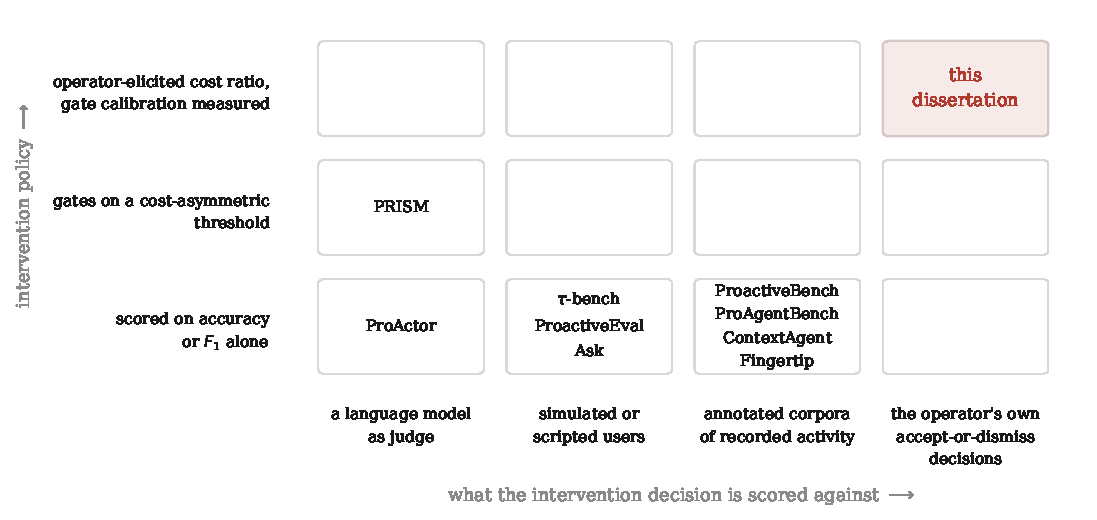
\includegraphics[width=\textwidth]{figures/gap_map}
  \caption[The surveyed proactive systems by intervention policy and by what
    their decisions are scored against]{%
    The proactive systems of Section~\ref{sec:rw-surfacing} placed on the two
    dimensions this chapter argues over: the policy by which a system decides
    to intervene, and what that decision is finally scored against. Columns run
    left to right by how directly the grounding is a real person's judgement.
    Every placement follows the citations in the surrounding text. PRISM
    \citep{fu_prism_2026} is alone in the middle row because it is the one
    surveyed system that gates on a calibrated acceptance probability rather
    than on accuracy alone, and it reports the gate's effect without reporting
    the calibration of the probability the gate depends on. The top-right cell
    is empty across the surveyed literature, which is where this dissertation
    sits; the emptiness is one of field instantiation and evaluation design,
    not of method. Peer-review status is not encoded here, being marked instead
    against each work where it is cited.}
  \label{fig:gap-map}
\end{figure}

The contribution is accordingly one of field instantiation, not of method.
\citet{paleyes_challenges_2022}'s survey is assembled from reports of systems in
deployment, a body of knowledge that exists because deployments were written up,
not because benchmarks were run. What is attempted here is to take a
risk-sensitive intervention policy of the kind PRISM specifies, place it above a
per-venue rhythm and a deviation signal defined by a calibrated band, and
evaluate the assembly against an operator's own decisions in a live multi-venue
setting. The rhythm is deliberately per-venue: cross-venue pooling is tested and
not adopted, which is the outcome the conjecture of
Section~\ref{sec:rw-rhythm} anticipates, so borrowing across venues is a
hypothesis this work examines rather than a component of the system it delivers.

Three limitations follow directly from the literature reviewed here and are
carried forward to the discussion of the work as a whole. The headline accuracy
figures are mean-absolute-scaled while Section~\ref{sec:rw-ruler} makes the case
for a squared-scaled measure; the expected calibration error that
Section~\ref{sec:rw-evaluation} identifies as the instrument capable of carrying
a coverage guarantee through to the agent's output is not computed anywhere in
this work; and the inter-demand interval estimated for each venue carries
sampling uncertainty Section~\ref{sec:rw-rhythm} leaves unquantified. Against the
three directions the literature does lead, pooling across three venues buying
little \citep{montero-manso_principles_2021}, a weather covariate having to earn
its place \citep{haben_short_2019,hertel_explainable_2026}, and a ranking
computed on a handful of origins carrying little information
\citep{hewamalage_look_2021,brigato_there_2025}, two of this project's
observations run the other way, and both are marked where they arise: the
direction of the ranking reversal in Section~\ref{sec:rw-ruler}, and the
performance of adaptive calibration at a regime change in
Section~\ref{sec:rw-deviation}. Whether a policy developed on annotated
benchmarks survives contact with one operator, three venues and a year of untidy
till data is the question this dissertation takes up.
